\pdfminorversion=7
% Options for packages loaded elsewhere
\PassOptionsToPackage{hyphens}{url}
%
\documentclass[sigconf, screen]{acmart}

\usepackage{xcolor}
%\usepackage{cleveref}
\usepackage{color}
\usepackage{fancyvrb}
\usepackage{acmart-taps}
\newcommand{\VerbBar}{|}
\newcommand{\VERB}{\Verb[commandchars=\\\{\}]}
\DefineVerbatimEnvironment{Highlighting}{Verbatim}{commandchars=\\\{\}}
% Add ',fontsize=\small' for more characters per line
\newenvironment{Shaded}{}{}
\newcommand{\AlertTok}[1]{\textcolor[rgb]{1.00,0.00,0.00}{\textbf{#1}}}
\newcommand{\AnnotationTok}[1]{\textcolor[rgb]{0.38,0.63,0.69}{\textbf{\textit{#1}}}}
\newcommand{\AttributeTok}[1]{\textcolor[rgb]{0.49,0.56,0.16}{#1}}
\newcommand{\BaseNTok}[1]{\textcolor[rgb]{0.25,0.63,0.44}{#1}}
\newcommand{\BuiltInTok}[1]{\textcolor[rgb]{0.00,0.50,0.00}{#1}}
\newcommand{\CharTok}[1]{\textcolor[rgb]{0.25,0.44,0.63}{#1}}
\newcommand{\CommentTok}[1]{\textcolor[rgb]{0.38,0.63,0.69}{\textit{#1}}}
\newcommand{\CommentVarTok}[1]{\textcolor[rgb]{0.38,0.63,0.69}{\textbf{\textit{#1}}}}
\newcommand{\ConstantTok}[1]{\textcolor[rgb]{0.53,0.00,0.00}{#1}}
\newcommand{\ControlFlowTok}[1]{\textcolor[rgb]{0.00,0.44,0.13}{\textbf{#1}}}
\newcommand{\DataTypeTok}[1]{\textcolor[rgb]{0.56,0.13,0.00}{#1}}
\newcommand{\DecValTok}[1]{\textcolor[rgb]{0.25,0.63,0.44}{#1}}
\newcommand{\DocumentationTok}[1]{\textcolor[rgb]{0.73,0.13,0.13}{\textit{#1}}}
\newcommand{\ErrorTok}[1]{\textcolor[rgb]{1.00,0.00,0.00}{\textbf{#1}}}
\newcommand{\ExtensionTok}[1]{#1}
\newcommand{\FloatTok}[1]{\textcolor[rgb]{0.25,0.63,0.44}{#1}}
\newcommand{\FunctionTok}[1]{\textcolor[rgb]{0.02,0.16,0.49}{#1}}
\newcommand{\ImportTok}[1]{\textcolor[rgb]{0.00,0.50,0.00}{\textbf{#1}}}
\newcommand{\InformationTok}[1]{\textcolor[rgb]{0.38,0.63,0.69}{\textbf{\textit{#1}}}}
\newcommand{\KeywordTok}[1]{\textcolor[rgb]{0.00,0.44,0.13}{\textbf{#1}}}
\newcommand{\NormalTok}[1]{#1}
\newcommand{\OperatorTok}[1]{\textcolor[rgb]{0.40,0.40,0.40}{#1}}
\newcommand{\OtherTok}[1]{\textcolor[rgb]{0.00,0.44,0.13}{#1}}
\newcommand{\PreprocessorTok}[1]{\textcolor[rgb]{0.74,0.48,0.00}{#1}}
\newcommand{\RegionMarkerTok}[1]{#1}
\newcommand{\SpecialCharTok}[1]{\textcolor[rgb]{0.25,0.44,0.63}{#1}}
\newcommand{\SpecialStringTok}[1]{\textcolor[rgb]{0.73,0.40,0.53}{#1}}
\newcommand{\StringTok}[1]{\textcolor[rgb]{0.25,0.44,0.63}{#1}}
\newcommand{\VariableTok}[1]{\textcolor[rgb]{0.10,0.09,0.49}{#1}}
\newcommand{\VerbatimStringTok}[1]{\textcolor[rgb]{0.25,0.44,0.63}{#1}}
\newcommand{\WarningTok}[1]{\textcolor[rgb]{0.38,0.63,0.69}{\textbf{\textit{#1}}}}
\setlength{\emergencystretch}{3em} % prevent overfull lines
\providecommand{\tightlist}{%
  \setlength{\itemsep}{0pt}\setlength{\parskip}{0pt}}
\setcounter{secnumdepth}{5}
\newlength{\cslhangindent}
\setlength{\cslhangindent}{1.5em}
\newlength{\csllabelwidth}
\setlength{\csllabelwidth}{3em}
\newlength{\cslentryspacingunit} % times entry-spacing
\setlength{\cslentryspacingunit}{\parskip}
\newenvironment{CSLReferences}[2] % #1 hanging-ident, #2 entry spacing
 {% don't indent paragraphs
  \setlength{\parindent}{0pt}
  % turn on hanging indent if param 1 is 1
  \ifodd #1
  \let\oldpar\par
  \def\par{\hangindent=\cslhangindent\oldpar}
  \fi
  % set entry spacing
  \setlength{\parskip}{#2\cslentryspacingunit}
 }%
 {}
\usepackage{calc}
\newcommand{\CSLBlock}[1]{#1\hfill\break}
\newcommand{\CSLLeftMargin}[1]{\parbox[t]{\csllabelwidth}{#1}}
\newcommand{\CSLRightInline}[1]{\parbox[t]{\linewidth - \csllabelwidth}{#1}\break}
\newcommand{\CSLIndent}[1]{\hspace{\cslhangindent}#1}

%\ifLuaTeX
%  \usepackage{selnolig}  % disable illegal ligatures
%\fi
%\usepackage[]{natbib}
%\IfFileExists{xurl.sty}{\usepackage{xurl}}{} % add URL line breaks if available
%\urlstyle{same} % disable monospaced font for URLs

\widowpenalty=10000
\clubpenalty=10000
\displaywidowpenalty=10000

\copyrightyear{2023}
\acmYear{2023}
\setcopyright{rightsretained}
\acmConference[IFL 2023]{The 35th Symposium on Implementation and Application of Functional Languages}{August 29--31, 2023}{Braga, Portugal}
\acmBooktitle{The 35th Symposium on Implementation and Application of Functional Languages (IFL 2023), August 29--31, 2023, Braga, Portugal}
\acmDOI{10.1145/3652561.3652565}
\acmISBN{979-8-4007-1631-7/23/08}
\keywords{dependent types, elaborators, elaboration, open datatype, extensible datatype, type-checking}

\begin{CCSXML}
<ccs2012>
   <concept>
       <concept_id>10011007.10011006.10011008.10011009.10011012</concept_id>
       <concept_desc>Software and its engineering~Functional languages</concept_desc>
       <concept_significance>500</concept_significance>
       </concept>
   <concept>
       <concept_id>10011007.10011074.10011075.10011077</concept_id>
       <concept_desc>Software and its engineering~Software design engineering</concept_desc>
       <concept_significance>300</concept_significance>
       </concept>
   <concept>
       <concept_id>10003752.10003790.10011740</concept_id>
       <concept_desc>Theory of computation~Type theory</concept_desc>
       <concept_significance>300</concept_significance>
       </concept>
   <concept>
       <concept_id>10002944.10011123.10011673</concept_id>
       <concept_desc>General and reference~Design</concept_desc>
       <concept_significance>100</concept_significance>
       </concept>
 </ccs2012>
\end{CCSXML}

\ccsdesc[500]{Software and its engineering~Functional languages}
\ccsdesc[300]{Software and its engineering~Software design engineering}
\ccsdesc[300]{Theory of computation~Type theory}
\ccsdesc[100]{General and reference~Design}


\begin{document}

\title{ExEl: Building an Elaborator Using Extensible Constraints}

\author{Bohdan Liesnikov}
\orcid{0009-0000-2216-8830}
\affiliation{
  \institution{Delft University of Technology}
  \city{Delft}
  \country{The Netherlands}}
\email{B.Liesnikov@tudelft.nl}
\author{Jesper Cockx}
\orcid{0000-0003-3862-4073}
\affiliation{
  \institution{Delft University of Technology}
  \city{Delft}
  \country{The Netherlands}}
\email{J.G.H.Cockx@tudelft.nl}

\hypersetup{
  pdftitle={ExEl: Building an Elaborator Using Extensible Constraints},
  pdfauthor={Bohdan Liesnikov and Jesper Cockx},
  pdfkeywords={dependent types, elaborators, elaboration, open datatype, extensible datatype, type-checking},
  pdfcreator={LaTeX via pandoc},
  pdfproducer={pdftex},
  hidelinks,
}

\begin{abstract}
  Proof assistants and dependently typed languages such as Coq, Agda, Lean, and Idris can be used to ascertain the correctness of software with mathematical precision.
  While much research has been done on their theoretical foundations, their actual implementations have been studied to a much lesser extent.
  As a result, features that are not considered part of the theoretical foundations - such as implicit arguments and type classes - have their own bespoke implementation for each language, making for code bases that are hard to understand and maintain.
  To address some of the common problems in the implementations of dependently typed languages, we present a modular architecture for implementing the transformation from user-friendly surface syntax into a small and well-behaved core language, also known as elaboration.
  Our architecture is made modular through the use of an open datatype of constraints and a plugin system for solvers that work on these constraints, which means that each new feature is contained in its own module.
  We showcase our design with a proof-of-concept elaborator for a language with dependent types, implicit arguments, higher-order unification, and instance arguments.
\end{abstract}


\maketitle


\hypertarget{sec:introduction}{%
\section{Introduction}\label{sec:introduction}}

Statically typed languages allow us to catch large classes of bugs at
compile-time by checking the implementation against its type signature.
When the types are provided by the user they can be viewed as a form of
specification, constraining the behaviour of the programs. This comes
with the benefit of more static guarantees but with an increased toll on
the user to supply more precise information about the program. Many
languages choose to infer types as a result, but another option is to
use the information in the types to infer parts of the program. This
idea was aptly worded by Conor McBride as ``Write more types and fewer
programs.''
\citetext{\citealp{ptoopTypeInferenceThought2022}; \citealp[chap.~2.1]{mcbrideEpigramPracticalProgramming2005}}
Some examples of this include overloaded functions in Java, implicits in
Scala, and type classes in Haskell.

In dependently typed languages like Agda
\citep{norellPracticalProgrammingLanguage2007, theagdateamAgdaUserManual2023a},
Coq \citep{thecoqdevelopmentteamCoqProofAssistant2022} or Idris
\citep{bradyIdrisGeneralpurposeDependently2013} the types can be much
more precise. This allows us to infer even larger parts of the program
from the type. Examples include implicit arguments in Agda, implicit
coercions in Coq, and tactic arguments in Idris. The inference of parts
of the program must not be fully automatic but can also be interactive
or partially automatic. Examples of interactive inference are holes in
Agda and proof obligations in Coq, while canonical structures
\citep{mahboubiCanonicalStructuresWorking2013} in Coq and
program-synthesis for holes in Haskell
\citep{koppelSearchingEntangledProgram2022} are partially automatic.

Each of these different inference features has its own algoritms and
extension points, which often evolved organically over time together
with the language, and are often not well isolated from each other. For
example, implicit arguments and instance search in Agda can interact in
unexpected ways \citep{agdausersPerformanceRegressionIssue2018}. Sized
types in Agda \citep{abelExtensionMartinLofType2016} also come with
their own solver that often interacts poorly with the regular solver for
implicit arguments. In Coq, canonical structures are notorious for
producing unpredictable results yet they were not properly documented
for 15 years \citep{mahboubiCanonicalStructuresWorking2013}. Lean 4 aims
to allow the users to develop new surface-level features
\citep{leonardodemouraLeanMetaprogramming2021} using elaboration monads
\citep{mouraLeanTheoremProver2021}, somewhat akin to elaborator
reflection in Idris
\citep{christiansenElaboratorReflectionExtending2016}, but Lean 3 was
built in a more conventional way \citep{demouraLeanTheoremProver2015}.
All these bespoke algorithms and their interactions put a toll on the
language developer to specify and implement them and on the user to
understand them.

The part of the implementation of a dependently typed language that is
responsible for type checking user-facing surface syntax and inferring
the parts that have been left implicit is known as the
\emph{elaborator}. One common piece of infrastructure used by
elaborators are metavariables, also known as ``existential variables''
\citep[chap.~2.2.1]{thecoqdevelopmentteamCoqProofAssistant2022}, which
represent as-of-yet unknown parts of the program. Together with
metavariables also comes unification, i.e.~the ability to constrain two
terms to be equal. Metavariables and unification are heavily used
throughout many elaborators for infering implicit arguments and for
general type-checking, making them sensitive towards changes in
unification algorithms. Because of the complexity unification, breaking
changes are often discovered only when run against a large existing
project on CI, such as the Standard and Cubical libraries for Agda or
the \texttt{unimath} library for Coq.

To move towards a cleaner and more maintainable model for implementing
elaborators, we propose a new architecture for an extensible elaborator
for dependently typed languages. Practically, our architecture allows
each feature to be contained within one module, as opposed to being
spread around the codebase. The implementations of the individual
features interact with the rest of the elaborator through an API for
providing new kinds of constraints and new solvers for these new
constraints as well as existing ones. This allows developers to put all
solvers related to one feature in one place, thus fulfilling our goal of
modularity. The design also separates the `what' the solvers are doing
from the `when', making the separation between different phases of
elaboration explicit. As a result, this allows the developer to reason
more easily about exceptions and asynchronicity during elaboration and
add new features in a more isolated fashion.

\textbf{Contributions}.

\begin{itemize}
\tightlist
\item
  We propose a new design blueprint for implementing an elaborator for a
  dependently typed language that is extensible with new constraints and
  new solvers. It supports type classes (Section
  \ref{sec:case-typeclasses}), implicit arguments (Section
  \ref{sec:case-implicits}), implicit coercions, and tactic arguments
  (Section \ref{sec:coercion-tactics}).
\item
  We propose a new view on metavariables as communication channels for
  the solvers, drawing parallels with asynchronous programming
  primitives (Section \ref{sec:solvers-implementation}).
\item
  We decompose the usual components of an elaborator, like the unifier
  in Agda, into a suite of solvers which can be extended and interleaved
  by user-provided plugins (Section
  \ref{sec:constraints_and_unification}).
\item
  Following the blueprint, we present a prototype implementation of a
  dependently typed language available at
  \href{https://github.com/liesnikov/extensible-elaborator}{github.com/liesnikov/extensible-elaborator}\footnote{Also archived at \href{https://doi.org/10.4121/e74fd14a-da79-4686-97e8-143ac5e0858d.v1}{doi.org/10.4121/e74fd14a-da79-4686-97e8-143ac5e0858d.v1}.}.
\end{itemize}

\hypertarget{sec:unification_constraint_based_elaboration_and_design_challanges}{%
\section{Unification, constraint-based elaboration and design
challenges}\label{sec:unification_constraint_based_elaboration_and_design_challanges}}

Constraints have been an integral part of compilers for strongly typed
languages for a long time \citep{oderskyTypeInferenceConstrained1999}.
For example, the implementations of both Haskell
\citep{vytiniotisOutsideInModularType2011} and Agda \citep[
chap.~3]{norellPracticalProgrammingLanguage2007} use constraints
extensively. In the former case, they are even reflected and can be
manipulated by the user
\citetext{\citealp[chap.~6.10.3]{orchardHaskellTypeConstraints2010a}; \citealp{ghcdevelopmentteamGHCUserGuide2022}}.
This has proven to be a good design decision for GHC, as is reflected
for example in a talk by \citet{peytonjonesTypeInferenceConstraint2019},
as well as in a few published sources
\citep{vytiniotisOutsideInModularType2011, peytonjonesPracticalTypeInference2007}.

In the land of dependently typed languages constraints are often used in
a much less principled manner. Agda has a family of constraints that
grew organically, currently counting 19 constructors.\footnote{\href{https://github.com/agda/agda/blob/v2.6.4/src/full/Agda/TypeChecking/Monad/Base.hs\#L1157-L1191}{./src/full/Agda/TypeChecking/Monad/Base.hs\#L1157-L1191}.
  Here and henceforth we shorten the links in footnotes to paths in the
  repository, the source code can be found at
  \href{https://github.com/agda/agda/blob/v2.6.4/}{github.com/agda/agda/blob/v2.6.4/}.}
Idris technically has constraints, with the only two constructors being
equality constraints for two terms and for two sequences of
terms.\footnote{\href{https://github.com/idris-lang/Idris2/blob/e673d05a67b82591131e35ccd50fc234fb9aed85/src/Core/UnifyState.idr}{./src/Core/UnifyState.idr}
  at\\
  \href{https://github.com/idris-lang/Idris2/blob/e673d05a67b82591131e35ccd50fc234fb9aed85}{github.com/idris-lang/Idris2/blob/e673d0}}
The same holds for Lean.\footnote{\href{https://github.com/leanprover/lean4/blob/0a031fc9bbb43c274bb400f121b13711e803f56c/src/Lean/Meta/Match/Basic.lean\#L161}{./src/Lean/Meta/Match/Basic.lean\#L161}
  at\\
  \href{https://github.com/leanprover/lean4/blob/0a031fc9bbb43c274bb400f121b13711e803f56c/}{github.com/leanprover/lean4/blob/0a031f}}
These languages either use constraints in a restricted, single-use-case
manner -- namely, for unification -- or in an ad-hoc manner.

In this section, we demonstrate why a more methodical approach to
constraints results in more robust elaborators across the board. In
particular, we go over three typical challenges that come up when
building a compiler for a dependently typed language and the way they
are usually solved: the complexity of managing a global state of
metavariables for unification (Section \ref{sec:conversion_checking}),
dealing with different kinds of implicit arguments and their solvers
(\ref{sec:implicit-arguments}), and user-facing extension points to
unification (Section \ref{sec:extending-unification}).

\hypertarget{sec:conversion_checking}{%
\subsection{Unification in the presence of
meta-variables}\label{sec:conversion_checking}}

As mentioned in the introduction, in the process of type-checking we use
unification to compare terms. The unification algorithms are often one
of the most complex parts of a type checker, which stems from the desire
of compiler writers to implement the most powerful unifier while being
limited by the fact that higher-order unification is undecidable in
general. Some of this complexity is unavoidable, but we can manage it
better by splitting up the unifier into smaller modular parts. In
practice, this means that one does not have to fit together an
always-growing unifier but can instead write different unification rules
separately.

As a real-world example, Agda's unification algorithm for solving
implicit arguments is spread between about a hundred functions and 2200
lines of code\footnote{\href{https://github.com/agda/agda/blob/v2.6.4/src/full/Agda/TypeChecking/Conversion.hs}{./src/full/Agda/TypeChecking/Conversion.hs}}.
Each of the functions implements part of the ``business logic'' of the
unifier, but a large part of their implementation is just there to deal
with bookkeeping related to metavariables and constraints:

\begin{enumerate}
\def\labelenumi{\arabic{enumi}.}
\tightlist
\item
  They throw and catch exceptions, driving the control flow of the
  unification.
\item
  They compute blockers that determine when a postponed constraint
  should be re-tried.
\item
  They have special cases for when either or both of the sides equation
  or its type are metavariables, or for when they are terms whose
  evaluation is blocked on some metavariables.
\end{enumerate}

Concretely, this code uses functions like \texttt{noConstraints},
\texttt{dontAssignMetas}, \texttt{catchConstraint}, and
\texttt{patternViolation} which rely on specific behaviour of the
constraint solver. Other functions like \texttt{reduceB} and
\texttt{abortIfBlocked} force the programmer to choose between letting
the constraint system handle blockers or doing it manually. These things
are known to be brittle and pose an increased mental overhead when
making changes, with a corresponding risk of introducing new bugs.

The unifier is called from many places throughout the type-checker: when
checking applications of variables and defined functions, type
annotations on lambda expressions, forced `dot' patterns, macro calls,
and various primitive operations of Cubical Agda. At the same time, it
is unintuitive and full of intricacies as indicated by multiple
comments\footnote{\href{https://github.com/agda/agda/blob/v2.6.4/src/full/Agda/TypeChecking/Conversion.hs\#L484-L485}{./src/full/Agda/TypeChecking/Conversion.hs\#\#L484-L485},
  \href{https://github.com/agda/agda/blob/v2.6.4/src/full/Agda/TypeChecking/Conversion.hs\#L541-L549}{./src/full/Agda/TypeChecking/Conversion.hs\#L541-L549}}.

We would like the compiler-writer to be able to separate managing
constraints and blockers from the actual logic of the comparison
function. If we zoom in on the \texttt{compareAtom} function, the core
logic can be expressed in about 20 lines\footnote{\href{https://github.com/agda/agda/blob/v2.6.4/src/full/Agda/TypeChecking/Conversion.hs\#L550-L599}{./src/full/Agda/TypeChecking/Conversion.hs\#L550-L599}}
of simplified code (ignoring advanced features like sized types,
cumulativity, polarity, and forcing). This is precisely what we would
like the developer to write.

\begin{imageonly}
\begin{Shaded}
\begin{Highlighting}[]
\KeywordTok{case}\NormalTok{ (m, n) }\KeywordTok{of}
\NormalTok{  (}\DataTypeTok{Lit}\NormalTok{ l1, }\DataTypeTok{Lit}\NormalTok{ l2) }\OperatorTok{|}\NormalTok{ l1 }\OperatorTok{==}\NormalTok{ l2 }\OtherTok{{-}\textgreater{}} \FunctionTok{return}\NormalTok{ ()}
\NormalTok{  (}\DataTypeTok{Var}\NormalTok{ i es, }\DataTypeTok{Var}\NormalTok{ i\textquotesingle{} es\textquotesingle{}) }\OperatorTok{|}\NormalTok{ i }\OperatorTok{==}\NormalTok{ i\textquotesingle{} }\OtherTok{{-}\textgreater{}} \KeywordTok{do}
\NormalTok{      a }\OtherTok{\textless{}{-}}\NormalTok{ typeOfBV i}
\NormalTok{      compareElims [] [] a (var i) es es\textquotesingle{}}
\NormalTok{  (}\DataTypeTok{Con}\NormalTok{ x ci xArgs, }\DataTypeTok{Con}\NormalTok{ y \_ yArgs) }\OperatorTok{|}\NormalTok{ x }\OperatorTok{==}\NormalTok{ y }\OtherTok{{-}\textgreater{}} \KeywordTok{do}
\NormalTok{      t\textquotesingle{} }\OtherTok{\textless{}{-}}\NormalTok{ conType x t}
\NormalTok{      compareElims t\textquotesingle{} (}\DataTypeTok{Con}\NormalTok{ x ci []) xArgs yArgs}
  \OperatorTok{...}
\end{Highlighting}
\end{Shaded}
\end{imageonly}

The functions described above are specific to Agda but in other major
languages we can find similar problems with unifiers being large pieces
of code that are hard to understand. The sizes of modules with unifiers
are as follows: Idris has 1.5kloc\footnote{\href{https://github.com/idris-lang/Idris2/blob/102d7ebc18a9e881021ed4b05186cccda5274cbe/src/Core/Unify.idr}{./src/Core/Unify.idr}}
of unification code, Lean 1.8kloc\footnote{\href{https://github.com/leanprover/lean4/blob/75252d2b85df8cb9231020a556a70f6d736e7ee5/src/Lean/Meta/ExprDefEq.lean}{./src/Lean/Meta/ExprDefEq.lean}},
and Coq 1.8kloc\footnote{\href{https://github.com/coq/coq/blob/b35c06c3ab3ed4911311b4a9428a749658d3eff1/pretyping/evarconv.mli}{./pretyping/evarconv.mli}
  at
  \href{github.com/coq/coq/blob/b35c06c3ab3ed4911311b4a9428a749658d3eff1/}{github.com/coq/coq/blob/b35c06}}.
For Haskell, which is not a dependently typed language yet, but does
have a constraints system
\citep{peytonjonesTypeInferenceConstraint2019}, this number is at
2kloc\footnote{\href{https://gitlab.haskell.org/ghc/ghc/-/blob/b81cd709df8054b8b98ac05d3b9affcee9a8b840/compiler/GHC/Core/Unify.hs}{./compiler/GHC/Core/Unify.hs}
  at\\
  \href{https://gitlab.haskell.org/ghc/ghc/-/blob/b81cd709df8054b8b98ac05d3b9affcee9a8b840}{gitlab.haskell.org/ghc/ghc/-/blob/b81cd709d}}.

\hypertarget{sec:implicit-arguments}{%
\subsection{Type-checking function application in the presence of
implicit arguments}\label{sec:implicit-arguments}}

During the type-checking of function application, there may be different
kinds of implicit arguments to infer, for example, instance arguments,
or tactic arguments. If we start from a simple case of type-checking an
application of a function symbol to regular arguments, every next
extension needs to be handled as a special case.

Take Agda -- when checking an application of a function with implicit
arguments\footnote{\href{https://github.com/agda/agda/blob/v2.6.4/src/full/Agda/TypeChecking/Implicit.hs\#L96-L128}{./src/full/Agda/TypeChecking/Implicit.hs\#L96-L128}}
we already have to carry the information on how the arguments will be
resolved (e.g.~through instance search) and then create a specific kind
of metavariable\footnote{\href{https://github.com/agda/agda/blob/v2.6.4/src/full/Agda/TypeChecking/Implicit.hs\#L130-L149}{./src/full/Agda/TypeChecking/Implicit.hs\#L130-L149}}
\citep[chap.~3]{norellPracticalProgrammingLanguage2007} for each of
those cases.

For handling \texttt{auto} variables, Idris 2
\citep[chap.~13.1]{theidristeamIdrisTutorial2021} has to essentially
inline the search procedure through a chain of elaboration function
calls (\texttt{checkApp} to \texttt{checkAppWith} to
\texttt{checkAppWith\textquotesingle{}}) to
\texttt{makeAutoImplicit}\footnote{\href{https://github.com/idris-lang/Idris2/blob/870bc824371d504a03af937f326216302210a875/src/TTImp/Elab/App.idr\#L224-L241}{./src/TTImp/Elab/App.idr\#L224-L241}}.
This can accommodate interfaces (or type classes), but one can imagine
that if a different kind of implicit was added, like tactic arguments or
canonical structures, we would have to inline the search again,
requiring a non-trivial modification to the elaboration mechanism.

While the codebases above show that it is certainly possible to extend
languages with new features if the language was not written with
extensibility in mind, this can lead to rather ad hoc solutions.

\hypertarget{sec:extending-unification}{%
\subsection{Extending unification}\label{sec:extending-unification}}

While writing a unifier is hard enough as it is, at times the developers
might want to give their users the ability to extend the unification
procedure.

Canonical structures
\citep{saibiOutilsGeneriquesModelisation1999, mahboubiCanonicalStructuresWorking2013}
are one example as they are in the overlap between type classes and
unification hints. Adding them to a language that does not support them
requires an extension of the unification algorithm with a rule that says
that projection from a canonical structure is injective \citep[eq.
1]{mahboubiCanonicalStructuresWorking2013}.

One could also provide means to do so manually in a more general case,
by allowing users to declare certain symbols as injective. This is one
of the features requested by the Agda users
\citep{agdausersInjectiveUnificationPragma2023}.

Another example of user-extensible unification can be found in
extensions with rules for associativity and commutativity, as described
in the thesis by \citet{holtenDependentTypeCheckingModulo2023}. It
required changes to 2000 lines of code\footnote{\href{https://github.com/LHolten/agda-commassoc/tree/defenitional-commutativity}{github.com/LHolten/agda-commassoc/tree/defenitional-commutativity}
  (sic)}. We would like to make changes such as this more feasible.

\hypertarget{sec:summary-of-the-issues}{%
\subsection{Summary of the issues}\label{sec:summary-of-the-issues}}

The examples above show that when building a dependently typed language
the core might be perfectly elegant and simple, but the features that
appear on top of it complicate the design. While the code in existing
implementations often relies on constraints, the design at large does
not put them at the centre of the picture and instead views them
primarily as a gadget. For example, Agda's constraint solver\footnote{\href{https://github.com/agda/agda/blob/v2.6.4/src/full/Agda/TypeChecking/Constraints.hs\#L247-L298}{src/full/Agda/TypeChecking/Constraints.hs\#L247-L298}}
relies on the type-checker to call it at the point where it is needed
and has to be carefully engineered to work with the rest of the
codebase.

\hypertarget{sec:what-is-our-design-bringing-into-the-picture}{%
\section{A blueprint for extensible
elaborators}\label{sec:what-is-our-design-bringing-into-the-picture}}

Our idea for a new design is to shift focus more towards the constraints
themselves:

\begin{enumerate}
\def\labelenumi{\arabic{enumi}.}
\item
  We give an API for raising constraints that can be called by the
  type-checker, essentially creating an ``ask'' to be fulfilled by the
  solvers. This is similar to the idea of mapping object-language
  unification variables to host-language ones as done by
  \citet{guidiImplementingTypeTheory2017}, the view of the ``asks'' as a
  general effect \citep[chap.~4.4]{bauerEqualityCheckingGeneral2020}, or
  the communication between actors
  \citep{allaisTypOSOperatingSystem2022a}.
\item
  To make the language more modular, we make constraints an extensible
  data type and give an API to define new solvers with the ability to
  specify what kinds of constraints they can solve. Since we're working
  in Haskell we encode constraints in the style of Data types à la carte
  \citep{swierstraDataTypesCarte2008}.
\end{enumerate}

In the examples in this paper, we follow the bidirectional style of
type-checking. In practice, however, the design decisions are agnostic
of the underlying system, as long as it adheres to the principle of
stating the requirements on terms in terms of raising a constraint and
not by, say, pattern-matching on a concrete term representation.

\begin{figure*}
  \center
  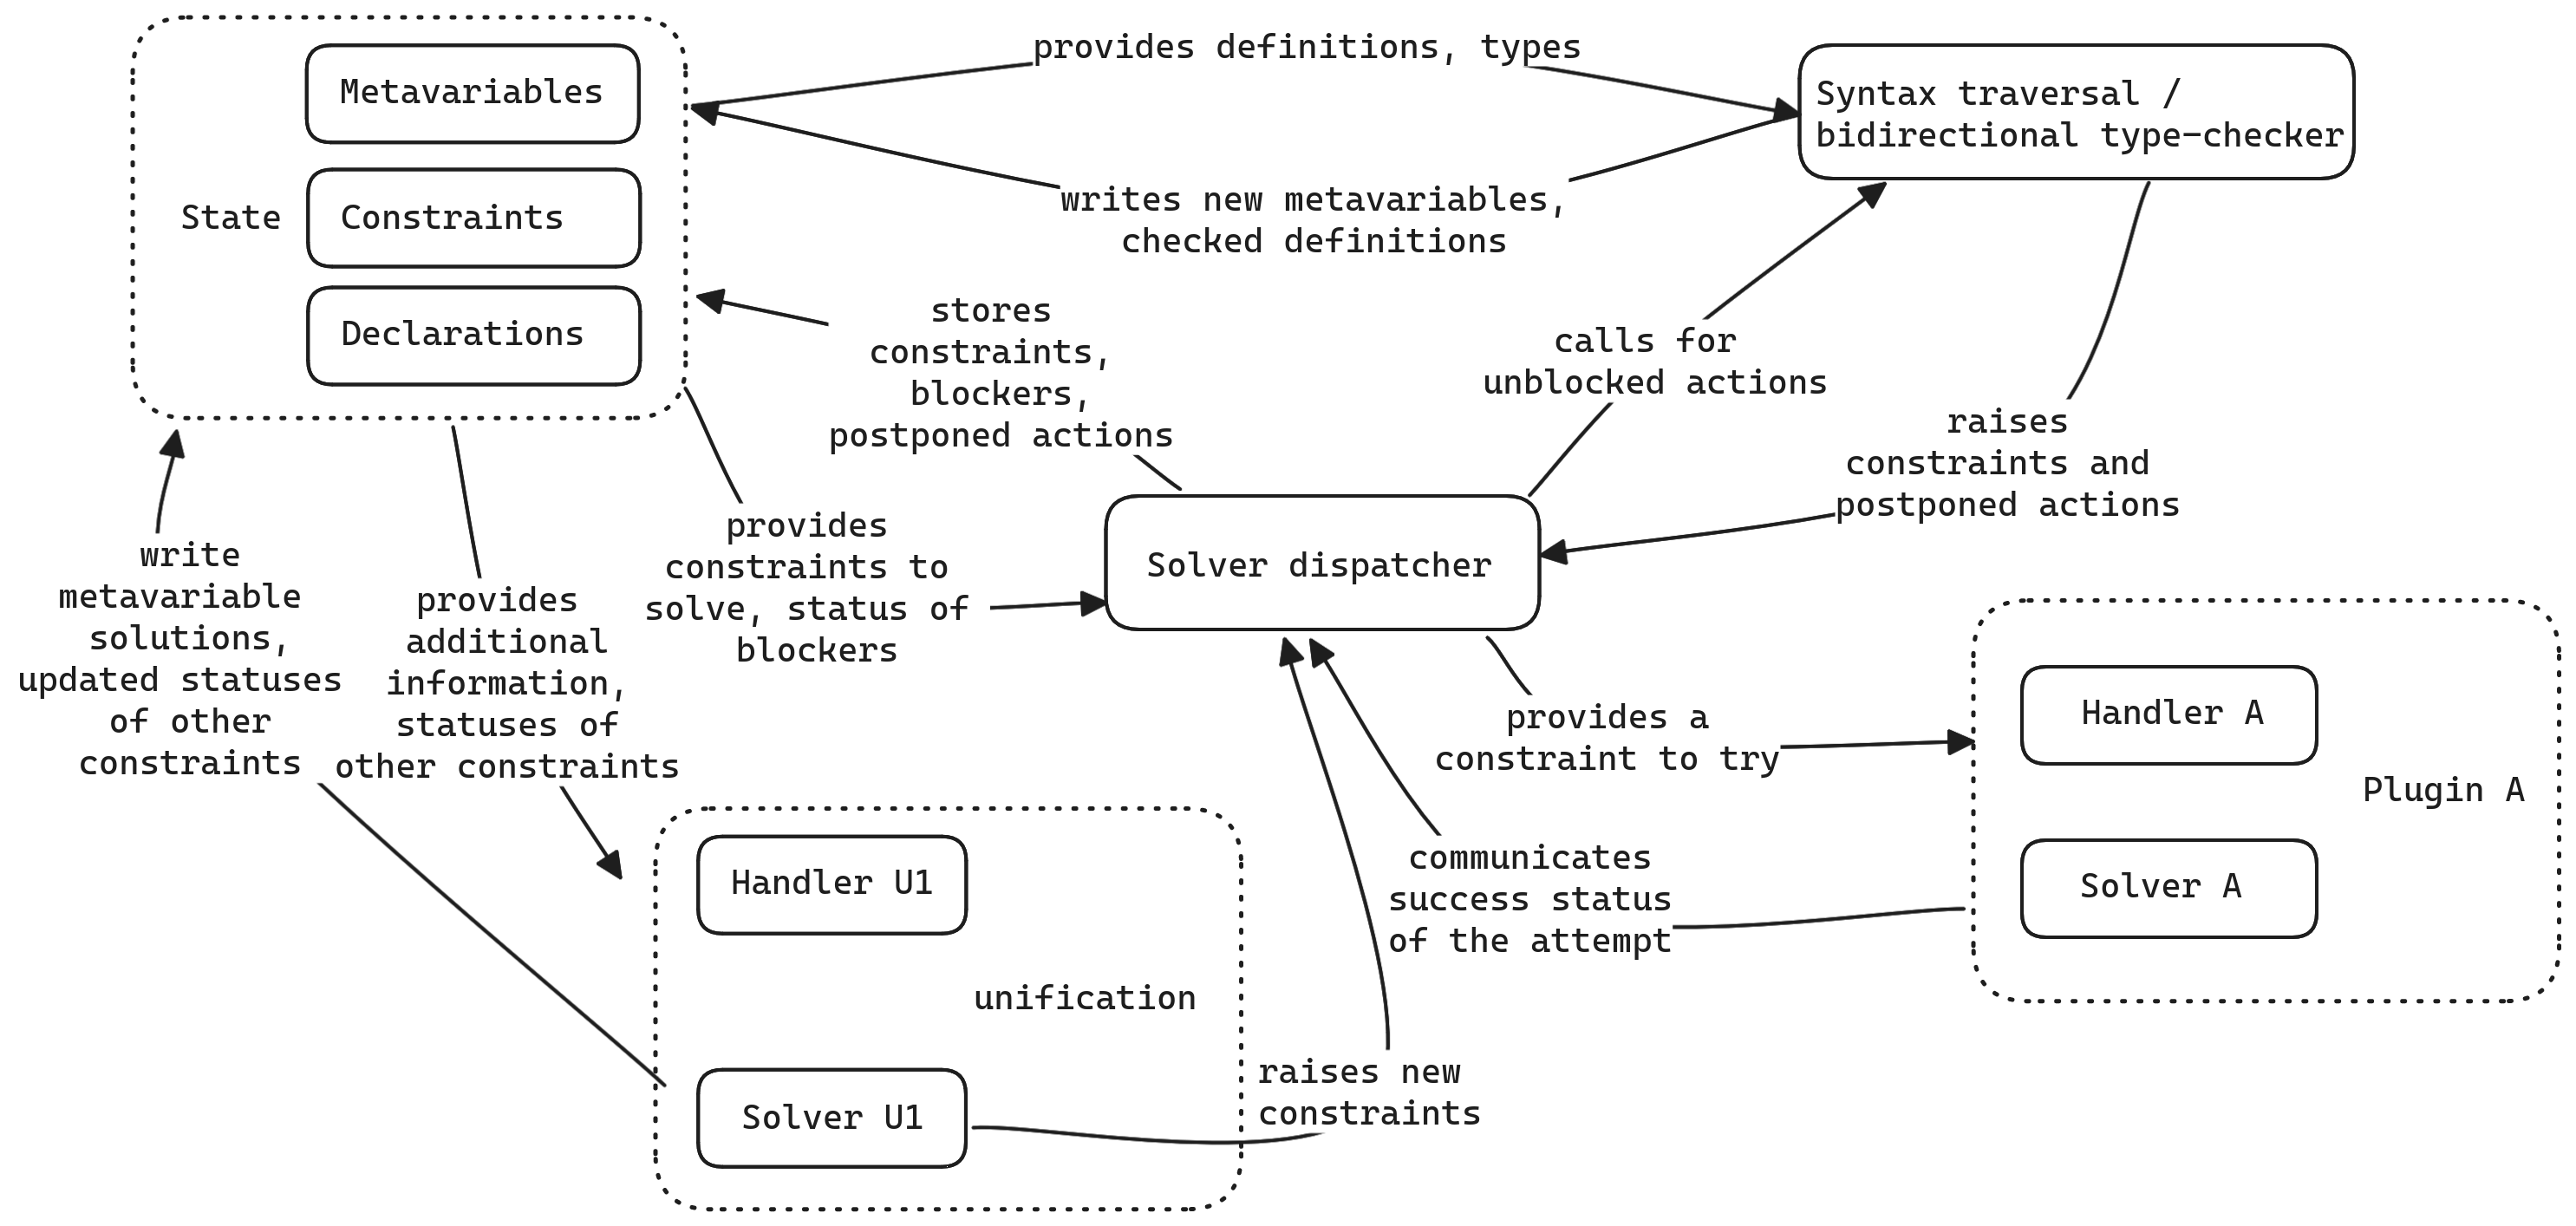
\includegraphics[width=\textwidth]{architecture-diagram}
  \caption{Architecture diagram}
  \label{architecture-figure}
\end{figure*}

From a birds-eye view, the architecture looks as depicted in Figure
\ref{architecture-figure}. Its main characteristics are the separation
of plugins/unification into independent pieces and a clear boundary
between solver dispatcher and the rest of the system.

Let us walk through each part of the architecture in more detail. The
type-checking begins by initializing the state and traversing the
syntax. The traversal raises the constraints, and for the moment, the
constraints are simply stored. As soon as we finish the traversal of a
block (one declaration in our case), the solver dispatcher is called. It
traverses the set of constraints, and tries to solve each active
constraint by making calls to different plugins. Each plugin, whether
user-supplied (\texttt{Plugin\ A}) or provided by us
(\texttt{unification}) consists of a handler and a solver. The handler
determines if the plugin can potentially solve a constraint, if so, the
dispatcher runs the corresponding solver.

All components have some read access to the state, including handlers
which might for example verify that there are no extra constraints on
the metavariable. For the write access: syntax traversal writes new
metavariables to the state and elaborated definitions; the solver
dispatcher writes updated meta-information; solvers write solutions to
the metavariables and can raise new constraints.

For the moment we need to recompile the project to include new plugins.
This is not necessity and a system that dynamically loads plugins is
possible to implement in a way that is similar to GHC Plugins\footnote{\href{https://mpickering.github.io/plugins.html}{mpickering.github.io/plugins.html}}
or Accelerate\footnote{\href{https://github.com/tmcdonell/accelerate-llvm/blob/master/accelerate-llvm-native/src/Data/Array/Accelerate/LLVM/Native/Link/Runtime.hs\#L40}{github.com/tmcdonell/accelerate-llvm/blob/master/accelerate-llvm-native/src/Data/Array/Accelerate/LLVM/Native/Link/Runtime.hs}}
\citep{mcdonellTypesafeRuntimeCode2015}.

\hypertarget{sec:bidirectional}{%
\section{Dependently typed calculus and bidirectional
typing}\label{sec:bidirectional}}

Now that we have described our architecture, we will demonstrate its
design through a practical implementation. First, in this section, we
describe the core of the type system we implement. The following
sections will then describe the constraints and their solvers. We take
pi-forall \citep{weirichImplementingDependentTypes2022} as a basis for
the system and extend it with metavariables in the core syntax and
implicit arguments in the surface syntax. However, for all other
purposes, we leave the core rules intact and, therefore, the core
calculus too.

\hypertarget{basic-language-and-rules}{%
\subsection{Basic language and rules}\label{basic-language-and-rules}}

This is a dependently typed calculus that includes Pi, Sigma and indexed
inductive types.

Here is the internal syntax term data type, apart from service
constructor omissions, like a placeholder \texttt{TRUSTME}.

\begin{imageonly}
\begin{Shaded}
\begin{Highlighting}[]
\KeywordTok{data} \DataTypeTok{Term} \OtherTok{=}
  \CommentTok{{-}{-} type of types Type}
    \DataTypeTok{Type}
  \CommentTok{{-}{-} variables x}
  \OperatorTok{|} \DataTypeTok{Var} \DataTypeTok{TName}
  \CommentTok{{-}{-} abstraction \textbackslash{}x. a}
  \OperatorTok{|} \DataTypeTok{Lam}\NormalTok{ (}\DataTypeTok{Bind} \DataTypeTok{TName} \DataTypeTok{Term}\NormalTok{)}
  \CommentTok{{-}{-} application a b}
  \OperatorTok{|} \DataTypeTok{App} \DataTypeTok{Term} \DataTypeTok{Arg}
  \CommentTok{{-}{-} function type (x : A) {-}\textgreater{} B}
  \OperatorTok{|} \DataTypeTok{Pi} \DataTypeTok{Type}\NormalTok{ (}\DataTypeTok{Bind} \DataTypeTok{TName} \DataTypeTok{Type}\NormalTok{)}
  \CommentTok{{-}{-} Sigma{-}type \{ x : A | B \}}
  \OperatorTok{|} \DataTypeTok{Sigma} \DataTypeTok{Term}\NormalTok{ (}\DataTypeTok{Bind} \DataTypeTok{TName} \DataTypeTok{Term}\NormalTok{)}
  \OperatorTok{|} \DataTypeTok{Prod} \DataTypeTok{Term} \DataTypeTok{Term}
  \OperatorTok{|} \DataTypeTok{LetPair} \DataTypeTok{Term}\NormalTok{ (}\DataTypeTok{Bind}\NormalTok{ (}\DataTypeTok{TName}\NormalTok{, }\DataTypeTok{TName}\NormalTok{) }\DataTypeTok{Term}\NormalTok{)}
  \CommentTok{{-}{-} Equality type  a = b}
  \OperatorTok{|} \DataTypeTok{TyEq} \DataTypeTok{Term} \DataTypeTok{Term}
  \OperatorTok{|} \DataTypeTok{Refl}
  \OperatorTok{|} \DataTypeTok{Subst} \DataTypeTok{Term} \DataTypeTok{Term}
  \OperatorTok{|} \DataTypeTok{Contra} \DataTypeTok{Term}
  \CommentTok{{-}{-} inductive datatypes}
  \OperatorTok{|} \DataTypeTok{TCon} \DataTypeTok{TCName}\NormalTok{ [}\DataTypeTok{Arg}\NormalTok{] }\CommentTok{{-}{-} types (fully applied)}
  \OperatorTok{|} \DataTypeTok{DCon} \DataTypeTok{DCName}\NormalTok{ [}\DataTypeTok{Arg}\NormalTok{] }\CommentTok{{-}{-} terms (fully applied)}
  \OperatorTok{|} \DataTypeTok{Case} \DataTypeTok{Term}\NormalTok{ [}\DataTypeTok{Match}\NormalTok{]}
    \CommentTok{{-}{-} metavariables}
  \OperatorTok{|} \DataTypeTok{MetaVar} \DataTypeTok{MetaClosure}
\end{Highlighting}
\end{Shaded}
\end{imageonly}

Equality is not defined as a regular inductive type but is instead
built-in. The user has access to the type and term constructor, but not
the ability to pattern-match on it. Instead, the language provides a
\texttt{subst} primitive of type
\texttt{(A\ x)\ -\textgreater{}\ (x=y)\ -\textgreater{}\ A\ y} and
\texttt{contra} that takes an equality of two different constructors of
an inductive type and produces an element of any type.

On top of the above, the language includes indexed inductive datatypes
and case-constructs for their elimination. Indexed inductive datatypes
are encoded as parameterised datatypes with an equality argument
constraining the index, also known as ``Henry Ford'' equality
\citep{chapmanGentleArtLevitation2010a}.

As for metavariables \texttt{MetaVar}: as mentioned in the introduction,
they are placeholders in the syntax tree (AST) that are produced in the
process of elaboration. Metavariables do not appear in the surface
syntax as they are not created by the user. In this paper we implement
metavariables in the contextual style, as described by
Abel and Pientka \cite{abelHigherOrderDynamicPattern2011}, therefore they are paired
with a closure of type \texttt{MetaClosure}.

\hypertarget{syntax-traversal}{%
\subsection{Syntax traversal}\label{syntax-traversal}}

We implement the core of the elaborator as a bidirectional syntax
traversal, raising a constraint every time we need to assert something
about the type.

This includes the expected use of unification constraints, for example
the case when we enter checking mode with a term whose type can be
inferred:

\begin{imageonly}
\begin{Shaded}
\begin{Highlighting}[]
\NormalTok{checkType tm ty }\OtherTok{=} \KeywordTok{do}
\NormalTok{  (etm, ty\textquotesingle{}) }\OtherTok{\textless{}{-}}\NormalTok{ inferType tm}
\NormalTok{  constrainEquality ty\textquotesingle{} ty }\DataTypeTok{I.Type}
  \FunctionTok{return}\NormalTok{ etm}
\end{Highlighting}
\end{Shaded}
\end{imageonly}

It also includes any time we want to decompose the type provided in
checking mode we pose a constraint that guarantees the type being in a
specific shape:

\begin{imageonly}
\begin{Shaded}
\begin{Highlighting}[]
\NormalTok{checkType (}\DataTypeTok{S.Lam}\NormalTok{ lam) ty }\OtherTok{=} \KeywordTok{do}
\NormalTok{  mtyA }\OtherTok{\textless{}{-}}\NormalTok{ createMetaTerm}
\NormalTok{  mtx }\OtherTok{\textless{}{-}}\NormalTok{ createUnknownVar}
  \CommentTok{{-}{-} extend the context with a new variable signature}
\NormalTok{  mtyB }\OtherTok{\textless{}{-}}\NormalTok{ extendCtx (}\DataTypeTok{I.TypeSig}\NormalTok{ (}\DataTypeTok{I.Sig}\NormalTok{ mtx mtyA))}
\NormalTok{                    (createMetaTerm)}
  \CommentTok{{-}{-} metaPi is the shape we want ty to be in}
  \KeywordTok{let}\NormalTok{ metaPi }\OtherTok{=} \DataTypeTok{I.Pi}\NormalTok{ mtyA (bind mtx mtyB)}

\NormalTok{  constrainEquality ty metaPi }\DataTypeTok{I.Type}
  \CommentTok{{-}{-} rest of the traversal can now use mtyA and mbnd}
  \OperatorTok{...}
\end{Highlighting}
\end{Shaded}
\end{imageonly}

At certain points, we have to raise a constraint which has an associated
continuation. For example, when checking the type of a data constructor,
the part of the program that comes as an argument to
\texttt{constrainTConAndFreeze} will be suspended (or ``blocked'') until
the meta is solved with something of the shape \texttt{TCon\ \_\ \_}.

\begin{imageonly}
\begin{Shaded}
\begin{Highlighting}[]
\NormalTok{checkType t}\OperatorTok{@}\NormalTok{(}\DataTypeTok{S.DCon}\NormalTok{ c args) ty }\OtherTok{=} \KeywordTok{do}
\NormalTok{  elabpromise }\OtherTok{\textless{}{-}}\NormalTok{ createMetaTerm}
\NormalTok{  constrainTConAndFreeze ty }\OperatorTok{$} \KeywordTok{do}
\NormalTok{    mty }\OtherTok{\textless{}{-}}\NormalTok{ substMetas ty}
    \KeywordTok{case}\NormalTok{ mty }\KeywordTok{of}
\NormalTok{      (}\DataTypeTok{I.TCon}\NormalTok{ tname params) }\OtherTok{{-}\textgreater{}} \KeywordTok{do}
        \OperatorTok{...}
\NormalTok{      \_ }\OtherTok{{-}\textgreater{}} \FunctionTok{error} \StringTok{"impossible"}
\end{Highlighting}
\end{Shaded}
\end{imageonly}

We add one more case to the elaborator for implicit arguments of any
kind, as will be described in more detail in Section
\ref{sec:case-implicits}.

\begin{imageonly}
\begin{Shaded}
\begin{Highlighting}[]
\NormalTok{checkType (}\DataTypeTok{Implicit}\NormalTok{) ty }\OtherTok{=} \KeywordTok{do}
\NormalTok{  m }\OtherTok{\textless{}{-}}\NormalTok{ createMetaTerm}
\NormalTok{  raiseConstraint }\OperatorTok{$} \DataTypeTok{FillInTheMeta}\NormalTok{ m ty}
  \FunctionTok{return}\NormalTok{ m}
\end{Highlighting}
\end{Shaded}
\end{imageonly}

As we see, the syntax traversal does not need to know anything about how
implicit arguments are resolved. The only thing we require is that the
elaboration of the argument is called with the type information
available. This corresponds to how, in bidirectional typing, function
application is done in the inference mode but the arguments are
processed in checking mode.

\begin{imageonly}
\begin{Shaded}
\begin{Highlighting}[]
\NormalTok{inferType (}\DataTypeTok{App}\NormalTok{ t1 t2) }\OtherTok{=} \KeywordTok{do}
\NormalTok{  (et1, }\DataTypeTok{Pi}\NormalTok{ tyA tyB) }\OtherTok{\textless{}{-}}\NormalTok{ inferType t1}
\NormalTok{  et2 }\OtherTok{\textless{}{-}}\NormalTok{ checkType t2 tyA}
  \FunctionTok{return}\NormalTok{ (}\DataTypeTok{App}\NormalTok{ et1 et2, subst tyB et2)}
\end{Highlighting}
\end{Shaded}
\end{imageonly}
\hypertarget{sec:constraints_and_unification}{%
\section{Constraints and
unification}\label{sec:constraints_and_unification}}

In Section \ref{sec:bidirectional} we described the syntax traversal
part of the elaborator, which generates the constraints. In this
section, we will go over the constraint datatype needed for the base
language, how unification is implemented and how we can extend the
unification procedure.

\hypertarget{base-constraints}{%
\subsection{Base constraints}\label{base-constraints}}

The datatype of constraints is open, which means the user can write a
plugin to extend it. However, we offer a few constraints out of the box
to be able to type-check the base language. For the base language, it
suffices to have the following:

\begin{itemize}
\item
  A constraint that enforces equality of two terms of a given type


\begin{imageonly}
\begin{Shaded}
\begin{Highlighting}[]
\CommentTok{{-}{-} two terms given should be equal}
\KeywordTok{data} \DataTypeTok{EqualityConstraint}\NormalTok{ e }\OtherTok{=}
     \DataTypeTok{EqualityConstraint} \DataTypeTok{Term} \DataTypeTok{Term} \DataTypeTok{Type} \DataTypeTok{MetaVarId}
\end{Highlighting}
\end{Shaded}
\end{imageonly}

  Here, \texttt{MetaVarId} refers to the anti-unification variable (see
  Section \ref{sec:solvers-implementation}).
\item
  A constraint that ensures that a metavariable is resolved eventually:

\begin{imageonly}
\begin{Shaded}
\begin{Highlighting}[]
\CommentTok{{-}{-} this terms has to be filled in}
\KeywordTok{data} \DataTypeTok{FillInTheTerm}\NormalTok{ e }\OtherTok{=}
     \DataTypeTok{FillInTheTerm} \DataTypeTok{Term}\NormalTok{ (}\DataTypeTok{Maybe} \DataTypeTok{Type}\NormalTok{)}
\end{Highlighting}
\end{Shaded}
\end{imageonly}
\item
  Lastly, a constraint which ensures that a term is a type constructor:

\begin{imageonly}
\begin{Shaded}
\begin{Highlighting}[]
\CommentTok{{-}{-} the term passed to the constraint}
\CommentTok{{-}{-} should be a type constructor}
\KeywordTok{data} \DataTypeTok{TypeConstructorConstraint}\NormalTok{ e }\OtherTok{=}
     \DataTypeTok{TypeConstructorConstraint} \DataTypeTok{Type}
\end{Highlighting}
\end{Shaded}
\end{imageonly}
\end{itemize}

The type-checker raises constraints and supplies the necessary
information in the process, but it is agnostic of how they will be
solved. In all of the examples above, the parameter \texttt{e} is
spurious. The need for this parameter comes from the technique we use to
encode open datatypes, and other constraint types can use it to encode
recursive occurrences of the constraints.

\hypertarget{sec:solvers-interface}{%
\subsection{Interface of the solvers}\label{sec:solvers-interface}}

On the solver side, we provide a suite\footnote{In the prototype we
  implement a subset of all unification rules, specifically:
  \texttt{identityPlugin}, \texttt{propagateMetasEqPlugin},
  \texttt{reduceLeftPlugin}, \texttt{reduceRightPlugin},
  \texttt{leftMetaPlugin}, \texttt{rightMetaPlugin},
  \texttt{typeConstructorPlugin},
  \texttt{typeConstructorWithMetasPlugin},
  \texttt{piEqInjectivityPlugin}, \texttt{tyEqInjectivityPlugin},
  \texttt{consInjectivityPlugin}, \texttt{typeInjectivityPlugin},
  \texttt{unificationStartMarker}, and \texttt{unificationEndMarker}.}
of solvers for unification that handle different cases of the problem.
The most basic plugin is the \texttt{syntactic} plugin which resolves
equality constraints where both sides are syntactically equal.

\begin{imageonly}
\begin{Shaded}
\begin{Highlighting}[]
\CommentTok{{-}{-} solves syntactically equal terms}
\OtherTok{syntacticHandler ::}\NormalTok{ (}\DataTypeTok{EqualityConstraint} \OperatorTok{:\textless{}:}\NormalTok{ c)}
                 \OtherTok{=\textgreater{}} \DataTypeTok{HandlerType}\NormalTok{ c}
\NormalTok{syntacticHandler constr }\OtherTok{=} \KeywordTok{do}
  \KeywordTok{let}\NormalTok{ eqcm }\OtherTok{=}\NormalTok{ match }\OperatorTok{@}\DataTypeTok{EqualityConstraint}\NormalTok{ constr}
  \KeywordTok{case}\NormalTok{ eqcm }\KeywordTok{of}
    \CommentTok{{-}{-} check for alpha{-}equality}
    \DataTypeTok{Just}\NormalTok{ (}\DataTypeTok{EqualityConstraint}\NormalTok{ t1 t2 ty \_) }\OtherTok{{-}\textgreater{}}
      \FunctionTok{return} \OperatorTok{$}\NormalTok{ aeq t1 t2}
    \DataTypeTok{Nothing} \OtherTok{{-}\textgreater{}}
      \FunctionTok{return} \DataTypeTok{False}
\OtherTok{syntacticSolver ::}\NormalTok{ (}\DataTypeTok{EqualityConstraint} \OperatorTok{:\textless{}:}\NormalTok{ c)}
                \OtherTok{=\textgreater{}} \DataTypeTok{SolverType} \DataTypeTok{Bool}
\OtherTok{syntactic ::} \DataTypeTok{Plugin}
\NormalTok{syntactic  }\OtherTok{=} \DataTypeTok{Plugin}\NormalTok{ \{ solver  }\OtherTok{=}\NormalTok{ syntacticSolver}
\NormalTok{                    , handler }\OtherTok{=}\NormalTok{ syntacticHandler}
                    \OperatorTok{...}
\NormalTok{                    \}}
\end{Highlighting}
\end{Shaded}
\end{imageonly}

We first define the class of constraints that will be handled by the
solver via providing a ``handler'' -- a function that decides whether a
given solver has to fire.\footnote{The code shown above and in the rest
  of the paper is close to the actual implementation, but has been
  simplified for presentation purposes. \texttt{HandlerType\ a} and
  \texttt{SolverType\ a} both morally correspond to
  \texttt{(ConstraintF\ cs)\ -\textgreater{}\ SolverMonad\ Bool}.} In
this case, this amounts to checking that the constraint given is indeed
an \texttt{EqualityConstraint} and that the two terms given to it are
syntactically equal. Then we define the solver itself. In this case does
not have to do anything except return \texttt{True} to indicate that the
constraint is solved. This is because it shall only fire once it has
been cleared to do so by the handler and the equality has already been
checked. Finally, we register the solver by declaring it using a plugin
interface.

The reason for the separation between a decision procedure and the
execution of the solver is to ensure separation between a potentially
slow, effectful solving and fast read-only decision-making in the
handler. We opt for this division since handlers will be run on many
constraints that do not fit them, therefore any write effects would have
to be rolled back. Solvers, on the other hand, should only fire in cases
when we can reasonably hope that the constraint will be solved and the
effects will not have to be rolled back.

In a similar fashion, we define \texttt{leftMetaSolver} and
\texttt{rightMetaSolver}, which only work on problems where one of the
sides is a metavariable. Here the job of the solver is not as trivial --
it has to check that the type of the other side indeed matches the
needed one and then register the instantiation of the metavariable in
the state.

Since a single constraint can often be handled by multiple solvers, we
can provide priority preferences, using the \texttt{pre} and
\texttt{suc} fields of the plugin interface. They are used to indicate
whether the currently defined plugin should run before or after,
respectively, which other plugins. At the time of running the compiler,
these preferences are loaded into a big pre-order relation for all the
plugins, which is then linearised and used to guide the solving
procedure.


\begin{imageonly}
\begin{Shaded}
\begin{Highlighting}[]
\OtherTok{rightMetaPlugin ::}\NormalTok{ (}\DataTypeTok{EqualityConstraint} \OperatorTok{:\textless{}:}\NormalTok{ cs)}
                \OtherTok{=\textgreater{}} \DataTypeTok{Plugin}\NormalTok{ cs}
\NormalTok{rightMetaPlugin }\OtherTok{=}
  \DataTypeTok{Plugin}\NormalTok{ \{ handler }\OtherTok{=}\NormalTok{ rightMetaHandler}
\NormalTok{         , solver  }\OtherTok{=}\NormalTok{ rightMetaSolver}
\NormalTok{         , symbol  }\OtherTok{=}\NormalTok{ rightMetaSymbol}
\NormalTok{         , pre }\OtherTok{=}\NormalTok{ []}
\NormalTok{         , suc }\OtherTok{=}\NormalTok{ [leftMetaSymbol]}
\NormalTok{         \}}
\end{Highlighting}
\end{Shaded}
\end{imageonly}

\hypertarget{sec:solvers-implementation}{%
\subsection{Implementation of the solvers and unification
details}\label{sec:solvers-implementation}}

We implement a system close to the one described by
Abel and Pientka \cite{abelHigherOrderDynamicPattern2011}. We modularise the
implementation by mapping every function call in the simplification
procedure to a raised constraint and every simplification rule to a
separate solver. For example, the ``decomposition of functions''
\citep[fig.~2]{abelHigherOrderDynamicPattern2011} rule is translated to
the following implementation.


\begin{imageonly}
\begin{Shaded}
\begin{Highlighting}[]
\OtherTok{piEqInjectivityHandler ::}\NormalTok{ (}\DataTypeTok{EqualityConstraint} \OperatorTok{:\textless{}:}\NormalTok{ cs)}
                       \OtherTok{=\textgreater{}} \DataTypeTok{HandlerType}\NormalTok{ cs}
\NormalTok{piEqInjectivityHandler constr }\OtherTok{=} \KeywordTok{do}
  \KeywordTok{let}\NormalTok{ eqcm }\OtherTok{=}\NormalTok{ match }\OperatorTok{@}\DataTypeTok{EqualityConstraint}\NormalTok{ constr}
  \KeywordTok{case}\NormalTok{ eqcm }\KeywordTok{of}
    \DataTypeTok{Just}\NormalTok{ (}\DataTypeTok{EqualityConstraint}\NormalTok{ pi1 pi2 \_ \_) }\OtherTok{{-}\textgreater{}}
      \KeywordTok{case}\NormalTok{ (pi1, pi2) }\KeywordTok{of}
\NormalTok{        (}\DataTypeTok{I.Pi}\NormalTok{ \_ \_ \_, }\DataTypeTok{I.Pi}\NormalTok{ \_ \_ \_) }\OtherTok{{-}\textgreater{}} \FunctionTok{return} \DataTypeTok{True}
\NormalTok{        \_ }\OtherTok{{-}\textgreater{}} \FunctionTok{return} \DataTypeTok{False}
\NormalTok{    \_ }\OtherTok{{-}\textgreater{}} \FunctionTok{return} \DataTypeTok{False}
\end{Highlighting}
\end{Shaded}
\end{imageonly}

The handler is simply checking that both sides of the equality are
indeed Pi-types, and in case either of the matches fails, it will be
reported and the solver will not be fired. The \texttt{match} function
above comes from the open datatype of constraints
\citep[sec.~5]{swierstraDataTypesCarte2008}, checking if \texttt{constr}
can be projected from \texttt{cs} to \texttt{EqualityConstraint}.

Now let us take a look at the solver. The rule we are implementing here
states that two \(\Pi\)-types can only be equal if both the types of the
domains (\texttt{a1}, \texttt{a2}) and the co-domains (\texttt{b1},
\texttt{b2}) are equal.

\begin{imageonly}
\begin{Shaded}
\begin{Highlighting}[]
\OtherTok{piEqInjectivitySolver ::}\NormalTok{ (}\DataTypeTok{EqualityConstraint} \OperatorTok{:\textless{}:}\NormalTok{ cs)}
                      \OtherTok{=\textgreater{}} \DataTypeTok{SolverType}\NormalTok{ cs}
\NormalTok{piEqInjectivitySolver constr }\OtherTok{=} \KeywordTok{do}
  \KeywordTok{let}\NormalTok{ (}\DataTypeTok{Just}\NormalTok{ (}\DataTypeTok{EqualityConstraint}\NormalTok{ (}\DataTypeTok{I.Pi}\NormalTok{ a1 b1)}
\NormalTok{                                (}\DataTypeTok{I.Pi}\NormalTok{ a2 b2) \_ m)) }\OtherTok{=}
\NormalTok{        match }\OperatorTok{@}\DataTypeTok{EqualityConstraint}\NormalTok{ constr}
\NormalTok{  ma }\OtherTok{\textless{}{-}}\NormalTok{ constrainEquality a1 a2 }\DataTypeTok{I.Type}
\NormalTok{  (x, tyB1) }\OtherTok{\textless{}{-}}\NormalTok{ unbind b1}
\NormalTok{  (y, tyB2\textquotesingle{}) }\OtherTok{\textless{}{-}}\NormalTok{ unbind b2}
  \KeywordTok{let}\NormalTok{ tyB2 }\OtherTok{=}\NormalTok{ subst y (}\DataTypeTok{I.Var}\NormalTok{ x) tyB2\textquotesingle{}}
\NormalTok{      mat  }\OtherTok{=}\NormalTok{ I.identityClosure ma}
\NormalTok{  mb }\OtherTok{\textless{}{-}}\NormalTok{ extendCtx (}\DataTypeTok{I.TypeSig}\NormalTok{ (}\DataTypeTok{I.Sig}\NormalTok{ x e1 mat)) }\OperatorTok{$}
\NormalTok{                  constrainEquality tyB1 tyB2 }\DataTypeTok{I.Type}
  \KeywordTok{let}\NormalTok{ mbt }\OtherTok{=}\NormalTok{ bind x }\OperatorTok{$}\NormalTok{ I.identityClosure mb}
\NormalTok{  solveMeta m (}\DataTypeTok{I.Pi}\NormalTok{ mat mbt)}
  \FunctionTok{return} \DataTypeTok{True}
\end{Highlighting}
\end{Shaded}
\end{imageonly}

Following pi-forall, we use the unbound-generics\footnote{\href{https://hackage.haskell.org/package/unbound-generics-0.4.3}{hackage.haskell.org/package/unbound-generics-0.4.3}}
library to deal with the names and binders (\texttt{unbind},
\texttt{subst} functions). As it will fire after a handler returns
\texttt{True}, we can assume the pattern-matches will not fail.

First, we constrain the equality of the domain of the Pi-type:
\texttt{a1} and \texttt{a2}. The seemingly spurious metavariable
\texttt{ma} returned from this call serves as an anti-unification
\citep{pfenningUnificationAntiunificationCalculus1991} communication
channel. Every time an equality constraint is created we return a
metavariable that stands for the unified term. This metavariable is used
for unification problems that are created in the extended contexts -- in
this case second argument of the Pi-type, but also when solving
equalities concerning two data constructors. We do this to tackle the
``spine problem''
\citep[sec.~1.4]{victorlopezjuanPracticalHeterogeneousUnification2021}
-- as we operate according to the ``well-typed modulo constraints''
principle, essentially providing a placeholder that is guaranteed to
preserve well-typedness in the extended context.\footnote{\(\text{Tog}^{+}\)
  \citep{victorlopezjuanTog2020, victorlopezjuanPracticalHeterogeneousUnification2021}
  focuses on extending the unification algorithm for the case where two
  sides of equality might not be of the same type, which is also a
  problem relevant for us. Their main argument against the usage of
  anti-unification in Agda provided there is that it is bug-prone. We
  think that in Agda the problems were stemming from the fact that
  anti-unification was implemented separately from unification, in which
  case it is indeed hard to keep the two in sync. There is no such
  duplication in our case since unification and anti-unification are
  one.} Finally, \texttt{ma} has to be applied to a closure, which will
keep track of the delayed substitution.

Then we can constrain the co-domains of Pi-types in an extended context.
In case one of the solvers the constraints created in the extended
context might need to know the exact shape of \texttt{ma}, we can block
on the metavariable later, freezing the rest of the problem until it is
instantiated.

As for the actual unification steps, we implement them in a similar
fashion to the simplification procedure. For example,
\texttt{leftMetaSolver} below handles the case where the left-hand side
of an equality constraint is an unsolved meta:

\begin{imageonly}
\begin{Shaded}
\begin{Highlighting}[]
\OtherTok{leftMetaSolver ::}\NormalTok{ (}\DataTypeTok{EqualityConstraint} \OperatorTok{:\textless{}:}\NormalTok{ cs)}
               \OtherTok{=\textgreater{}} \DataTypeTok{SolverType}\NormalTok{ cs}
\NormalTok{leftMetaSolver constr }\OtherTok{=} \KeywordTok{do}
  \KeywordTok{let}\NormalTok{ (}\DataTypeTok{Just}\NormalTok{ (}\DataTypeTok{EqualityConstraint}\NormalTok{ t1 t2 \_ m)) }\OtherTok{=}
\NormalTok{        match }\OperatorTok{@}\DataTypeTok{EqualityConstraint}\NormalTok{ constr}
\NormalTok{      (}\DataTypeTok{MetaVar}\NormalTok{ (}\DataTypeTok{MetaVarClosure}\NormalTok{ m1 c1)) }\OtherTok{=}\NormalTok{ t1}
\NormalTok{  mt2 }\OtherTok{\textless{}{-}}\NormalTok{ occursCheck m1 t2}
  \KeywordTok{case}\NormalTok{ mt2 }\KeywordTok{of}
    \CommentTok{{-}{-} indicates a failure in occurs{-}check}
    \DataTypeTok{Left}\NormalTok{ e }\OtherTok{{-}\textgreater{}} \FunctionTok{return} \DataTypeTok{False}
    \CommentTok{{-}{-} indicates a passed occurs{-}check}
    \DataTypeTok{Right}\NormalTok{ t2 }\OtherTok{{-}\textgreater{}}
      \KeywordTok{case}\NormalTok{ (invertClosureOn c1 (freeVarList t2)) }\KeywordTok{of}
        \DataTypeTok{Just}\NormalTok{ s }\OtherTok{{-}\textgreater{}} \KeywordTok{do}
          \KeywordTok{let}\NormalTok{ st2 }\OtherTok{=}\NormalTok{ substs s t2}
          \CommentTok{{-}{-} apply the subsitution}
\NormalTok{          solveMeta m1 st2}
          \CommentTok{{-}{-} instantiate the anti{-}unification variable}
\NormalTok{          solveMeta m st2}
          \FunctionTok{return} \DataTypeTok{True}
        \DataTypeTok{Nothing} \OtherTok{{-}\textgreater{}} \FunctionTok{return} \DataTypeTok{False}
\end{Highlighting}
\end{Shaded}
\end{imageonly}

Once the occurs-check returns and if it was successful, we apply the
inverted closure to the right-hand side of the equality.

By splitting up the rules into individual, simple solvers we can
compartmentalise the complexity of the unifier, making sure that each
rule is as decoupled from the others as possible. This does not
deteriorate the properties of the system but does not help to enforce
them either. We talk more about the challenge of proving correctness in
Section \ref{sec:limitations}.

\hypertarget{extending-unification}{%
\subsection{Extending unification}\label{extending-unification}}

Now that unification is implemented let us create a simple plugin that
makes certain symbols declared by the user injective
\citep{agdausersInjectiveUnificationPragma2023}. The actual
implementation is relatively simple and is not dissimilar to the
Pi-injectivity solver we showed above.

\begin{imageonly}
\begin{Shaded}
\begin{Highlighting}[]
\OtherTok{userInjectivitySolver ::}\NormalTok{ (}\DataTypeTok{EqualityConstraint} \OperatorTok{:\textless{}:}\NormalTok{ cs)}
                      \OtherTok{=\textgreater{}} \DataTypeTok{SolverType}\NormalTok{ cs}
\NormalTok{userInjectivitySolver constr }\OtherTok{=} \KeywordTok{do}
  \KeywordTok{let}\NormalTok{ (}\DataTypeTok{Just} \DataTypeTok{EqualityConstraint}
\NormalTok{              (}\DataTypeTok{I.App}\NormalTok{ (}\DataTypeTok{I.Var}\NormalTok{ f) a)}
\NormalTok{              (}\DataTypeTok{I.App}\NormalTok{ (}\DataTypeTok{I.Var}\NormalTok{ g) b) \_ m)) }\OtherTok{=}
\NormalTok{        match }\OperatorTok{@}\DataTypeTok{EqualityConstraint}\NormalTok{ constr}
  \KeywordTok{if}\NormalTok{ f }\OperatorTok{==}\NormalTok{ g}
  \KeywordTok{then} \KeywordTok{do}
\NormalTok{    ifM (queryInjectiveDeclarations f)}
\NormalTok{        (}\KeywordTok{do}
\NormalTok{           ms }\OtherTok{\textless{}{-}}\NormalTok{ constrainEquality a b }\DataTypeTok{I.Type}
\NormalTok{           solveMeta m ms}
           \FunctionTok{return} \DataTypeTok{True}\NormalTok{)}
\NormalTok{        (}\FunctionTok{return} \DataTypeTok{False}\NormalTok{)}
  \KeywordTok{else} \FunctionTok{return} \DataTypeTok{False}
\end{Highlighting}
\end{Shaded}
\end{imageonly}

where \texttt{queryInjectiveDeclarations} simply scans the available
declarations for a marker that \texttt{f} has been declared injective.

The only big thing left is to make sure that this solver fires at the
right time. This can only conflict with the ``decomposition of
neutrals'' rule, so we indicate to the solver dispatcher that our plugin
should run before it:

\begin{imageonly}
\begin{Shaded}
\begin{Highlighting}[]
\OtherTok{userInjectivityPlugin ::}\NormalTok{ (}\DataTypeTok{EqualityConstraint} \OperatorTok{:\textless{}:}\NormalTok{ cs)}
                      \OtherTok{=\textgreater{}} \DataTypeTok{Plugin}\NormalTok{ cs}
\NormalTok{userInjectivityPlugin }\OtherTok{=}
  \DataTypeTok{Plugin}\NormalTok{ \{ }\OperatorTok{...}
\NormalTok{         , solver }\OtherTok{=}\NormalTok{ userInjectivitySolver}
\NormalTok{         , symbol }\OtherTok{=} \DataTypeTok{PluginId} \OperatorTok{$} \StringTok{"userInjectivity"}
\NormalTok{         , pre }\OtherTok{=}\NormalTok{ [ unifyNeutralsDecomposition}
\NormalTok{                 , unificationEndMarkerSymbol]}
\NormalTok{         , suc }\OtherTok{=}\NormalTok{ [unificationStartMarkerSymbol]}
\NormalTok{         \}}
\end{Highlighting}
\end{Shaded}
\end{imageonly}

This modification does not alter the core of the language.

\hypertarget{sec:casestudies}{%
\section{Case studies}\label{sec:casestudies}}

Once we implement basic elaboration and unification we can extend the
language. This is where we make use of the fact that the constraints
datatype is open.

We saw before in Section \ref{sec:implicit-arguments} that conventional
designs require separate handling of different kinds of implicit
variables. To simplify the design we would like to uniformly dispatch a
search for the solution, which would be handled by a fitting solver. We
can achieve this by communicating the kind of the meta through its type
in the second argument of \texttt{FillInTheMeta\ m\ ty}. The solvers
then match on the shape of the type of the metavariable and handle it in
a case-specific manner: instance-search for type classes, tactic
execution for a tactic argument, or waiting for regular unification to
solve the metavariable for regular implicit arguments.

In this section, we will describe the implementation details of regular
implicit arguments (Section \ref{sec:case-implicits}) and the
implementation of type classes added on top of the implicit arguments
(Section \ref{sec:case-typeclasses}). And finally (Section
\ref{sec:coercion-tactics}) we sketch the implementation of coercive
subtyping and tactic arguments.

\hypertarget{sec:case-implicits}{%
\subsection{Implicit arguments}\label{sec:case-implicits}}

As we mentioned, the rule for \texttt{Implicit} had to be added to the
syntax traversal part of the elaborator. In fact, we require not one but
two modifications that lie outside of the solvers-constraints part of
the system. The first one is, indeed, the addition of a separate case in
the syntax traversal, however contained. The second one lies in the
purely syntactical part of the compiler: we need the pre-processor to
insert the placeholder terms in the surface syntax.

In particular, we need to desugar declarations of functions in the
following way. For any declaration of a function with some implicit
arguments, we wrap the type of each implicit argument with an
\texttt{Implicit}:

\begin{verbatim}
def f : {A : Type} -> {a : A} -> B a -> C
\end{verbatim}

becomes

\begin{verbatim}
def f : (A : Implicit Type)
     -> (a : Implicit (deImp A))
     -> (b : B (deImp a)) -> C
\end{verbatim}

Then, for each function call we insert the corresponding number of
implicit arguments, for example transforming \texttt{f\ b1} to
\texttt{f\ \_\ \_\ b1}.

For basic usage of implicit arguments this suffices -- as soon as we
have the placeholders in the surface syntax we create the constraints in
the \texttt{Implicit} case of the syntax traversal. The only solver that
is needed in this case is a trivial one that checks that the
metavariable has been instantiated in the end. The actual solving in
this case is done by the unifier itself, and the constraint simply
serves as a way to guarantee that all implicits are eventually
instantiated.

\begin{imageonly}
\begin{Shaded}
\begin{Highlighting}[]
\OtherTok{fillInImplicitSymbol ::} \DataTypeTok{PluginId}

\OtherTok{fillInImplicitHandler ::}\NormalTok{ (}\DataTypeTok{FillInImplicit} \OperatorTok{:\textless{}:}\NormalTok{ cs)}
                      \OtherTok{=\textgreater{}} \DataTypeTok{HandlerType}\NormalTok{ cs}
\NormalTok{fillInImplicitHandler constr }\OtherTok{=} \KeywordTok{do}
  \KeywordTok{let}\NormalTok{ ficm }\OtherTok{=}\NormalTok{ match }\OperatorTok{@}\DataTypeTok{FillInImplicit}\NormalTok{ constr}
  \KeywordTok{case}\NormalTok{ ficm }\KeywordTok{of}
    \DataTypeTok{Just}\NormalTok{ (}\DataTypeTok{FillInImplicit}\NormalTok{ term ty) }\OtherTok{{-}\textgreater{}} \KeywordTok{do}
      \KeywordTok{case}\NormalTok{ term }\KeywordTok{of}
        \DataTypeTok{MetaVar}\NormalTok{ (}\DataTypeTok{MetaVarClosure}\NormalTok{ mid \_) }\OtherTok{{-}\textgreater{}}
\NormalTok{          isMetaSolved mid}
\NormalTok{        \_ }\OtherTok{{-}\textgreater{}} \FunctionTok{return} \DataTypeTok{False}
    \DataTypeTok{Nothing} \OtherTok{{-}\textgreater{}} \FunctionTok{return} \DataTypeTok{False}

\OtherTok{fillInImplicitPlugin ::}\NormalTok{ (}\DataTypeTok{FillInImplicit} \OperatorTok{:\textless{}:}\NormalTok{ cs)}
                     \OtherTok{=\textgreater{}} \DataTypeTok{Plugin}\NormalTok{ cs}
\NormalTok{fillInImplicitPlugin }\OtherTok{=} \DataTypeTok{Plugin}\NormalTok{ \{}
\NormalTok{    solver }\OtherTok{=}\NormalTok{ fillInImplicitSolver,}
\NormalTok{  , handler }\OtherTok{=}\NormalTok{ fillInImplicitHandler}
\NormalTok{  , symbol }\OtherTok{=}\NormalTok{ fillInImplicitSymbol}
\NormalTok{  , suc }\OtherTok{=}\NormalTok{ []}
\NormalTok{  , pre }\OtherTok{=}\NormalTok{ []}
\NormalTok{  \}}
\end{Highlighting}
\end{Shaded}
\end{imageonly}

There is a design choice to be made in the implementation of
\texttt{Implicit\ A} and \texttt{deImp}. One option is to turn them into
a constructor and a projection of a record type, and the other is to
make them computationally equivalent to \texttt{id}. In the former case,
we need to manually unwrap them both in the pre-processor and during the
constraint-solving, but since the head symbol is distinct we can
guarantee that other solvers will not match on it, unless explicitly
instructed to. In the latter case, one has to be cautious of the order
in which the solvers are activated, particularly in the case of
different search procedures, should they be implemented. However, in the
example above it does not make a difference.

A limitation of this scheme is that we can only support functions with
``obvious'' implicit arguments -- i.e.~those that appear syntactically
in the declaration of the function. This is due to the fact that
insertion of metavariables happens before any type information is
available. For this reason Haskell-like impredicativity
\citep{serranoQuickLookImpredicativity2020a} in type inference cannot be
supported. If a more comprehensive support for implicit arguments is
desired, our system could be extended with support for first-class
implicits \citep{kovacsElaborationFirstclassImplicit2020}.

\hypertarget{sec:case-typeclasses}{%
\subsection{Type classes}\label{sec:case-typeclasses}}

Next, let us implement a plugin that adds support for type classes by
means of instance arguments \citep{DevrieseP11-1}. As in the case for
implicit arguments in general, we rely again on a pre-processor to
insert placeholder arguments of type \texttt{Instance\ a} for each
instance argument of type \texttt{a}.

Let us start by going through an example of the elaboration process for
a simple term. For type classes we need a few declarations, listed below
in Agda-like syntax:

\begin{verbatim}
plus  :  {A : Type} -> {{PlusOperation A}}
     -> (a : A) -> (b : A) -> A

instance BoolPlus : PlusOperation Bool where
  plus = orb
\end{verbatim}

And the exemplary term itself is:

\begin{verbatim}
m = plus True False
\end{verbatim}

\begin{enumerate}
\def\labelenumi{\arabic{enumi}.}
\item
  First, the pre-processor eliminates the implicits and type class
  arguments. We end up with the following declarations:

\begin{verbatim}
plus : (impA : Implicit Type)
    -> Instance PlusOperation (deImp impA)
    -> (a : deImp impA) -> (b :  deImp impA)
    -> deImp impA

instanceBoolPlus : InstanceT PlusOperation Bool
instanceBoolPlus =
  InstanceC (TypeClassC (Plus orb))

m = plus _ _ True False
\end{verbatim}

  Turning the declaration \texttt{instance\ BoolPlus} into a usage of
  the constructor \texttt{InstanceC} is precisely the part we need the
  pre-processor to do.
\item
  Next, we go into the elaboration of \texttt{m}. The elaborator applies
  \texttt{inferType\ (App\ t1\ t2)} rule four times and
  \texttt{checkType\ (Implicit)\ ty} twice on the two placeholders. The
  output of the elaborator is

\begin{verbatim}
m = plus ?_1 ?_2 True False
\end{verbatim}

  The state of the elaborator now contains four constraints:

\begin{verbatim}
C1: FillInTheTerm ?_1 (Implicit Type)
C2: FillInTheTerm ?_2 (InstanceT PlusOperation
                                 (deImp ?_1))
C3: EqualityConstraint (deImp ?_1) Bool Type
C4: EqualityConstraint (deImp ?_1) Bool Type
\end{verbatim}

  The first two correspond to implicit arguments, while the latter two
  are unification problems rendered into constraints.
\item
  Now we step into the constraint-solving world. First, the unifier
  solves the latter two constraints, instantiating \texttt{?\_1} to
  \texttt{Implicit\ Bool}. \texttt{C1} is then discarded as solved since
  \texttt{?\_1} is already instantiated to \texttt{Implicit\ Bool}.
  Next, the type class resolution launches a search for the instance of
  type \texttt{Instance\ PlusOperation\ Bool}.
\item
  This is where the type class plugin can take over. It transforms
  \texttt{C2:\ FillInTheTerm\ ?\_2\ (InstanceT\ PlusOperation\ Bool)} to
  \texttt{C5:\ InstanceSearch\ PlusOperation\ Bool\ ?\_2}. \texttt{C5}
  then gets matched by the search plugin for concrete instances, simply
  weeding through available declarations, looking for something of the
  shape \texttt{InstanceT\ PlusOperation\ Bool}. Such a declaration
  exists indeed and we can instantiate \texttt{?\_2} to
  \texttt{instanceBoolPlus}.
\end{enumerate}

Now let us take a look at the plugin for the constraint system. It is
contained in a single file
\href{https://github.com/liesnikov/extensible-elaborator/blob/elaborator-experiments/exel/src/Plugins/Typeclasses.hs}{\texttt{./exel/src/Plugins/Typeclasses.hs}}.
In it, we define a new constraint type \texttt{InstanceSearch}, a solver
that transforms constraints of the shape
\texttt{FillInTheType\ ?\ (InstanceT\ \_)} to the new constraint, and
finally, a solver for instance search problems. The reason to transform
the original constraint to the new type is to ensure that no other
solver will make an attempt at this problem, therefore modulating
interactions with other plugins.

Finally, the implementation of search for concrete instances is quite
simple:

\begin{imageonly}
\begin{Shaded}
\begin{Highlighting}[]
\NormalTok{instanceConcreteSolver constr }\OtherTok{=} \KeywordTok{do}
  \KeywordTok{let}\NormalTok{ (}\DataTypeTok{Just}\NormalTok{ (}\DataTypeTok{InstanceSearch}\NormalTok{ tcn ty m)) }\OtherTok{=}
\NormalTok{        match }\OperatorTok{@}\DataTypeTok{InstanceSearch}\NormalTok{ constr}
\NormalTok{  alldecls }\OtherTok{\textless{}{-}}\NormalTok{ collectInstancesOf tcn }\OperatorTok{\textless{}$\textgreater{}}\NormalTok{ SA.getDecls}
\NormalTok{  sty }\OtherTok{\textless{}{-}}\NormalTok{ SA.substAllMetas ty}
  \KeywordTok{case}\NormalTok{ Map.lookup sty alldecls }\KeywordTok{of}
    \DataTypeTok{Just}\NormalTok{ i }\OtherTok{{-}\textgreater{}} \KeywordTok{do}
\NormalTok{      SA.solveMeta m (}\DataTypeTok{I.Var}\NormalTok{ i)}
      \FunctionTok{return} \DataTypeTok{True}
    \DataTypeTok{Nothing} \OtherTok{{-}\textgreater{}} \FunctionTok{return} \DataTypeTok{False}
\end{Highlighting}
\end{Shaded}
\end{imageonly}

We conjecture that implementation of canonical structures
\citep{mahboubiCanonicalStructuresWorking2013} would be relatively
simple in such a system due to the openness of both unification
procedure and instance search.

\hypertarget{sec:coercion-tactics}{%
\subsection{Tactic arguments and coercions}\label{sec:coercion-tactics}}

In a similar fashion to the transformation of the
\texttt{FillInImplicit} constraints to \texttt{InstanceSearch}, we can
implement plugins for tactic arguments and coercive subtyping.

The former would be quite similar to what we saw in the previous section
\ref{sec:case-typeclasses}, except we would have to resolve
\texttt{FillInImplicit} to a \texttt{RunTactic} constraint (or run the
tactic directly). The question of how to actually run the tactics is
independent of the constraint machinery, noting that we allow for
running arbitrary type-checking actions during solving of constraints.

Coercive subtyping is of a slightly different nature. First, it would be
the most reliant on a pre-processor out of all of the examples described
above, since coercions could potentially be inserted around each
function argument, and potentially also around heads of applications and
types of abstractions \citep{tassiBiDirectionalRefinementAlgorithm2012}.
However, blindly inserting placeholders for coercions in every position
leads to constraints that cannot be resolved locally. Consider the
following example:

\begin{verbatim}
f : (A : Type) -> A -> A
arg : ArgTy

t : ExpTy
t = f _ arg
\end{verbatim}

This declaration would desugar to

\begin{verbatim}
t = coerce _ (f _ (coerce _ arg))
\end{verbatim}

which gives rise to two constraints, where \texttt{Coercion\ A\ B}
stands for the evidence of \texttt{A} being a subtype of \texttt{B}:

\begin{verbatim}
C1 : Coercion ArgTy ?1
C3 : Coercion ?1 ExpTy
\end{verbatim}

Clearly, we can not solve the first constraint in isolation and need to
consider all coercion constraints related to a particular type at the
same time. Hence this feature would be anti-modular in the sense that in
order to side-step the conflict between inference and coercions the
solver would need to look at the whole graph of subtyping constraints at
the same time. While we can accommodate such solvers, due to solvers
having write access to the state, it becomes much harder to modulate
interactions between different plugins. It also comes with a potential
performance penalty, which we describe further in Section
\ref{sec:limitations}.

\hypertarget{sec:limitations}{%
\section{Limitations}\label{sec:limitations}}

While our design offers a lot of flexibility, it does not solve every
problem. In this section, we describe a few examples of extensions that
do not quite fit in this framework as well as more general limitations.

\hypertarget{handling-of-meta-variables-outside-of-definition-sites}{%
\subsection{Handling of meta-variables outside of definition
sites}\label{handling-of-meta-variables-outside-of-definition-sites}}

After we elaborate a definition, there can still be unsolved
metavariables in it. This presents us with a design choice. The first
option is to generalize the definition over the metavariables and
instantiate them per-use site, essentially considering the metavariables
as additional (implicit) arguments to the definition. The second option
is to leave them up to be solved later, which might make elaboration
less predictable since now the use sites can influence whether a
particular definition type-checks. The third option is to freeze the
metavariables by considering them to be postulates, and report them as
an error at the end of type checking.

In particular, the second option allows us to incorporate more involved
inference algorithms into the system. For example, if we were to
implement an erasure inference algorithm as described by
Tejiščák \cite{tejiscakDependentlyTypedCalculus2020}, we would have to create
metavariable annotations (described as ``evars'' in the paper) that can
be instantiated beyond the definition site. The downside is that the
meaning of a definition can then change depending on where they are
used, making the outcome of elaboration depend on the file as a whole
rather than the definition itself.

\hypertarget{the-language-is-only-as-extensible-as-the-syntax-traversal-is}{%
\subsection{The language is only as extensible, as the syntax traversal
is}\label{the-language-is-only-as-extensible-as-the-syntax-traversal-is}}

Extensibility via constraints allows for a flexible user-specified
control flow as soon as we step into the constraints world. However, not
all features can be supported purely by adding constraints and solvers.
For example, consider the following simplified lambda-function
type-checking function\footnote{\href{https://github.com/agda/agda/blob/v2.6.4/src/full/Agda/TypeChecking/Rules/Term.hs\#L430-L518}{./src/full/Agda/TypeChecking/Rules/Term.hs\#L430-L518}}
from Agda:

\begin{imageonly}
\begin{Shaded}
\begin{Highlighting}[]
\NormalTok{checkLambda\textquotesingle{} cmp b xps typ body target }\OtherTok{=} \KeywordTok{do}
  \DataTypeTok{TelV}\NormalTok{ tel btyp }\OtherTok{\textless{}{-}}\NormalTok{ telViewUpTo numbinds target}
  \KeywordTok{if}\NormalTok{ size tel }\OperatorTok{\textless{}}\NormalTok{ numbinds }\OperatorTok{||}\NormalTok{ numbinds }\OperatorTok{/=} \DecValTok{1}
    \KeywordTok{then}\NormalTok{ dontUseTargetType}
    \KeywordTok{else}\NormalTok{ useTargetType tel btyp}
\end{Highlighting}
\end{Shaded}
\end{imageonly}

Here Agda steps away from the bidirectional discipline and infers a
(lambda) function if the target type is not fully known. In order to add
such a rule to our implementation, we would have to update syntax
traversal to be more flexible in where it allows lambda expressions to
appear. The solution, in this case, is effectively to replicate what
Agda is doing by implementing each type-checking rule in inference mode,
essentially factoring out \texttt{dontUseTargetType} in Agda's code
snippet above.

Likewise, implementing the commutativity and associativity unifier
plugins from Holten \cite{holtenDependentTypeCheckingModulo2023} requires
modifications in the core language, since we two terms that are equal
during elaboration have to equal during core type-checking too.

\hypertarget{lack-of-backtracking}{%
\subsection{Lack of backtracking}\label{lack-of-backtracking}}

We do not implement any backtracking in the solver dispatcher as it is
now. This means that every step taken is committing to a specific choice
to how to solve the constraint, which can be a limitation in cases where
one would like to have backtracking -- for example, Agda's instance
arguments search (with \texttt{-\/-overlapping-instances} flag)
\citep[chap.~3.18]{theagdateamAgdaUserManual2023a}, as well as type
classes in Lean \citep{selsamTabledTypeclassResolution2020}.

Backtracking in principle could be achieved by tracking changes to the
state of the elaborator and the production graph for constraints, but
such a system would be rather awkward. Alternatively, controlled
backtracking can be implemented within one solver, removing the
extension points, but allowing arbitrary control flow within the
algorithm.

\hypertarget{reliance-on-a-pre-processor}{%
\subsection{Reliance on a
pre-processor}\label{reliance-on-a-pre-processor}}

This work crucially relies on a pre-processor of some kind, be it macro
expansion or some other way to extend the parser with custom desugaring
rules. In particular, in order to implement n-ary implicit arguments
correctly and easily we need the pre-processor to expand them to the
right arity, similar to Matita
\citep[chap.~5]{tassiBiDirectionalRefinementAlgorithm2012} and others
\citep{serranoQuickLookImpredicativity2020a, kovacsElaborationFirstclassImplicit2020}.

\hypertarget{eager-reduction-and-performance}{%
\subsection{Eager reduction and
performance}\label{eager-reduction-and-performance}}

As the pre-processing step inserts a fair number of wrappers and
un-wrappers for all implicits and even more for coercions, we can expect
a performance penalty due to larger terms and spurious computation
steps. In particular, we expect this to be a major concern for coercive
subtyping.

As one possible mitigation, we suggest a discipline where constraint
solvers latch on to non-reduced types and terms in constraints. With
this discipline, we can borrow a trick from the implementation of Coq,
where the wrappers and unwrappers are identity functions and
\texttt{coerce\ f\ t} computes to \texttt{f\ t}. This also means that
constraints can/have to match on unreduced types in the
e.g.~\texttt{FillInTheTherm}.

In fact, we already use this trick to an extent for a different reason
-- since the calculus allows only fully applied type constructors, we
have to wrap each type class constructor in a lambda-abstraction for it
to appear as an argument to \texttt{TypeClassT\ typeClassName\ argType}.
Or, concretely, we have to define and use
\texttt{PlusOperation\textquotesingle{}\ =\ \textbackslash{}A\ .\ PlusOperation\ A}
in place of \texttt{PlusOperation} in the elaboration example in Section
\ref{sec:case-typeclasses}.

\hypertarget{proving-correctness}{%
\subsection{Proving correctness}\label{proving-correctness}}

As soon as we allow the users to implement their own solvers, there is
little we can say about the correctness of the system as a whole without
imposing proof obligations on the plugin writers. This is simply a
consequence of the fact that we do not invent a new unification
algorithm, but rather provide means of easier implementation for it. We
conjecture that our system satisfies the solution and type preservation
properties -- Theorems 2 and 3 from
Abel and Pientka \cite{abelHigherOrderDynamicPattern2011}, respectively -- assuming that
each solver on its own satisfies these properties. For termination the
situation is similar -- we conjecture that if every solver in the system
``reduces the weight'' of the unification problem, in terms of Theorem 1
by \citet{abelHigherOrderDynamicPattern2011}, we can guarantee
termination of the solving process as a whole.

\hypertarget{sec:related_work}{%
\section{Related work}\label{sec:related_work}}

We are certainly not the first ones to try to tackle the extensibility
of a language implementation. Dependently typed language implementations
usually consist of at least four parts: parser, elaborator, core
type-checker, and code generation backend. The code generation part is
currently irrelevant to our interests, since for a language to be
specified usually means for specification of the core, anything that
happens after the core does not extend the language, but rather tries to
preserve its semantics in some form. Therefore we're left with three
parts: parser, elaborator, and core type-checker.

We see parser or syntax extensibility as a necessary part of an
extensible language. This problem has been studied extensively in the
past and has a multitude of existing solutions. Macros are one of them
and are used heavily in various forms in many established languages
\citep{thecoqdevelopmentteamCoqProofAssistant2022, theagdateamAgdaUserManual2023a, ullrichNotationsHygienicMacro2020}
and can be powerful enough to build a whole language around
\citep{changDependentTypeSystems2019}.

Core extensibility, on the other hand, appears to be a problem with too
many degrees of freedom. Andromeda
\citep{bauerDesignImplementationAndromeda2018, bauerEqualityCheckingGeneral2020}
made an attempt at extensible definitional equality but is quite far
from a usable dependently typed language. Agda's philosophy allows
developers to experiment with the core but also results in a larger
amount of unexpected behaviours. In general, modifications of the core
rules will result in fundamental changes in the type theory, which can
break plenty of important properties like soundness or subject
reduction.

This leaves us with the question of the extensibility of an elaborator.
We will make a division here between syntax traversals, constraint
solving and all other features. The syntax traversal part of the
elaborator is relatively stable and commonly implemented following a
(roughly) bidirectional
discipline\citep{norellPracticalProgrammingLanguage2007, tassiBiDirectionalRefinementAlgorithm2012, ferreiraBidirectionalElaborationDependently2014},
so there seems little reason to make it extensible.

GHC has a plugin system that allows users to dynamically add custom
constraint solvers, but the type of constraints itself is not
extensible\footnote{\href{https://gitlab.haskell.org/ghc/ghc/-/wikis/plugins/type-checker/notes}{gitlab.haskell.org/ghc/ghc/-/wikis/plugins/type-checker/notes}}
\citep{peytonjonesTypeInferenceConstraint2019, vytiniotisOutsideInModularType2011, peytonjonesPracticalTypeInference2007}.

Coq \citep{thecoqdevelopmentteamCoqProofAssistant2022}, being one of the
most popular proof assistants, invested a lot effort into user-facing
features: work on tactics like a new tactic engine
\citep{spiwackVerifiedComputingHomological2011} and tactic languages
(Ltac2 \citep{pedrotLtac2TacticalWarfare2019}, SSReflect
\citep{gonthierSmallScaleReflection2008}, etc.), the introduction of a
virtual machine for performance
\citep{gregoireCompiledImplementationStrong2002} and others. However,
the implementation is quite hard to extend. One either has to modify the
source code, which is mostly limited to the core development team, as
seen from the
\href{https://github.com/coq/coq/graphs/contributors}{contributors
graph}, or one has to use Coq plugin system, which is rather
challenging, and in the end, the complexity of it gave rise to 
TemplateCoq/MetaCoq  \aptLtoX[graphic=no,type=html]{\cite{malechaExtensibleProofEngineering2014, sozeauMetaCoqProject2020}}{\citetext{\citealp[
]{malechaExtensibleProofEngineering2014}; \citealp{sozeauMetaCoqProject2020}}}.
While MetaCoq did open the possibility for some plugins
\citep{nielsenFormalisingDecentralisedExchanges2023, liesnikovGeneratingInductionPrinciples2020, forsterCertifyingExtractionTime2019}
to be written in a simpler way, their capabilities are still limited.

Agda has historically experimented a lot with different extensions to
both the type system and the elaborator, even though the design does not
accommodate these changes naturally. Instead, each of these extensions
is spread throughout many different parts of the code base\footnote{some
  recent examples:
  \href{https://github.com/agda/agda/pull/6385}{github.com/agda/agda/pull/6385},
  \href{https://github.com/agda/agda/pull/6354}{github.com/agda/agda/pull/6354}.}.

Lean introduced elaborator extensions
\citep{leonardodemouraLeanMetaprogramming2021, ullrichNotationsHygienicMacro2020}.
They allow the user to overload the commands, but if one defines a
particular elaborator it becomes hard to interleave with others. In a
way, this is an imperative view on extensibility.

Idris
\citep{bradyIdrisGeneralpurposeDependently2013, christiansenElaboratorReflectionExtending2016}
appeared as a programming language first and proof-assistant second and
does not provide either a plugin or hook system at all, except for
reflection. Idris also focuses on tactics as the main mechanism for
elaboration.

Turnstile+ by \citet{changDependentTypeSystems2019} uses macros to
elaborate surface syntax to a smaller core. Macros allow them to
modularly implement individual features, however combining different
features requires the user to re-define all macros from scratch. This is
the same problem as the one we mentioned for Lean.

TypOS \citep{allaisTypOSOperatingSystem2022a, guillaumeallaisTypOS2022}
is perhaps the closest to our work, but there are two important
differences. First, it is a domain-specific language for building
type-checkers, while our design is language-agnostic, as long as the
host language can model extensible datatypes in some capacity. Second,
their approach settles features of the language as they are decided by
the main developer and does not concern future changes and evolution.
Finally, we try to stay close to the designs of existing dependently
typed languages and offer flexibility in terms of choices, while TypOS
requires the developer to start from scratch and restricts certain
capabilities like overlapping rules for unification.

\hypertarget{future-work}{%
\section{Future work}\label{future-work}}

We see three main prospects for future work:

\begin{itemize}
\tightlist
\item
  \textbf{Exploration of different kinds of metavariables.} Currently,
  we implement metavariables only for terms, while for some applications
  such as erasure \citep{tejiscakDependentlyTypedCalculus2020} or
  irrelevance inference, it would be beneficial to have metavariables
  representing erasure and relevance annotations. Additionally, we can
  introduce metavariables for names and implement data constructor
  disambiguation more simply, which would remove the current need to
  block on the expected type of overloaded constructors.
\item
  \textbf{Rendering more elements of the elaborator as constraints.}
  Currently, components such as the occurs checking and reduction are
  simple function calls. Including them in the constraint machinery
  would make the implementation more uniform and allow users to extend
  them.
\item
  \textbf{Error messages} are not the focus of present work, but it
  would be interesting to see if we can incorporate ideas by
  \citet{heerenScriptingTypeInference2003} into our system.
\item
  \textbf{Potential optimisations}. Currently, our system has a lot of
  room for potential optimisations. The first step would be to allow
  handlers to pass some information to their respective solvers, which
  is conceptually an easy change but technically requires introduction
  of an existential type in the plugin. Additionally, some expandable
  per-plugin store for the solvers would be useful, for example, to
  avoid recompututation of type class instances on every invocation.
  Somewhat more ambitiously, one can imagine a caching system for
  constraints, avoiding the need for solving the same constraint more
  than once. In particular, caching of reduction seems like it would be
  beneficial since we currently do a lot of redundant computations.
  However, the memory usage of such a caching system might be
  prohibitive. Finally, we would also like to explore possibilities for
  concurrent solving, similar to the plans of
  \citet{allaisTypOSOperatingSystem2022a} to use LVars for representing
  metavariables \citep{kuperLatticebasedDataStructures2015}.
\end{itemize}

\hypertarget{refs}{}
\begin{CSLReferences}{0}{0}
\end{CSLReferences}

\begin{acks}
  Jesper Cockx holds an \grantsponsor{nwoviveni202216}{NWO Veni}{https://www.nwo.nl/en/projects/viveni202216} grant on `A trustworthy and extensible core language for Agda' (\href{https://www.nwo.nl/en/projects/viveni202216}{VI.Veni.202.216}).
\end{acks}
  
\bibliographystyle{ACM-Reference-Format}

\bibliography{bib.bib}

\end{document}